
%%%%%%%%%%%%%%%%%%%%%
\section{Champ d'altitude}
%%%%%%%%%%%%%%%%%%%%%
%
Les cartes topographiques représentent le "relief" grâce à des lignes "de même altitude".
Les {\it lignes de niveaux} sont une représentation du champ d'altitude.

\begin{center}
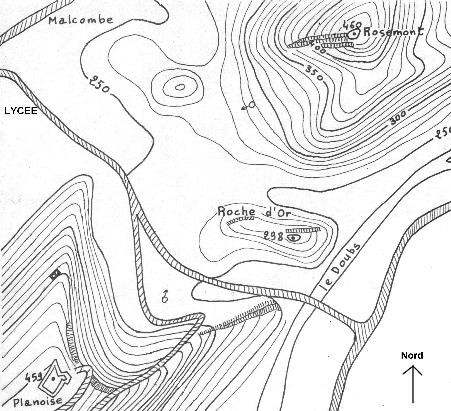
\includegraphics[scale=5]{./champs/topographique}
\end{center}

Ce champ ($A$) est une application qui associe une altitude ($z$) à chaque point ($x,y$) de la carte.

\begin{align*}
A :\ \ \ \ \ \ \ \ \mathbb{R} ^2 \ \  & \rightarrow \ \ \mathbb{R} \\
(x,y) \ \ & \mapsto \ \ z = A(x,y)
\end{align*}



%%%%%%%%%%%%%%%%%%%%%%%%%%%%%%%%%%%%%%%%%%%%%%%%%%%%%%%%%%%%%%%%%%%%%%%%%%%%
